\documentclass[tikz,border=8pt]{standalone}
% Shared look for every TikZ diagram. Load with \input{../../tools/tikz-style.tex}
\usepackage[T1]{fontenc}
\usepackage{lmodern}
\renewcommand{\sfdefault}{lmr}  % diagrams use the same serif as the text
\usetikzlibrary{arrows.meta, positioning, shapes.geometric, calc, fit, backgrounds}
\definecolor{cblue}{HTML}{4C78A8}
\definecolor{corange}{HTML}{F58518}
\definecolor{cgreen}{HTML}{54A24B}
\definecolor{cred}{HTML}{E45756}
\definecolor{cpurple}{HTML}{B279A2}
\definecolor{cgrey}{HTML}{6B6B6B}
\tikzset{
  every picture/.style={font=\sffamily, line width=1.2pt},
  box/.style={draw=#1, fill=#1!12, rounded corners=4pt, align=center, inner sep=7pt, minimum height=1.1cm},
  box/.default=cgrey,
  arrow/.style={-{Stealth[length=3mm]}, draw=cgrey, line width=1.4pt},
  title/.style={font=\sffamily\bfseries\Large},
  note/.style={font=\sffamily\small, text=cgrey, align=center},
}
\AtBeginDocument{\hyphenpenalty=10000 \exhyphenpenalty=10000}

% All 16 ways to fill 4 cells along a beam (1 = something blocks the cell, 0 = free), grouped by the FIRST
% blocked cell. First blocked at cell 1: 8 strings; cell 2: 4; cell 3: 2; cell 4: 1; none blocked: 1.
\newcommand{\cellrow}[2]{% #1 = x offset, #2 = y; draws 4 cells from \bits
  \foreach \b [count=\i] in \bits {
    \ifnum\b=1 \fill[corange!80] (#1+\i*0.42-0.42,#2) rectangle ++(0.38,0.32);
    \else \draw[cgrey!60, line width=0.8pt] (#1+\i*0.42-0.42,#2) rectangle ++(0.38,0.32); \fi }}
\begin{document}
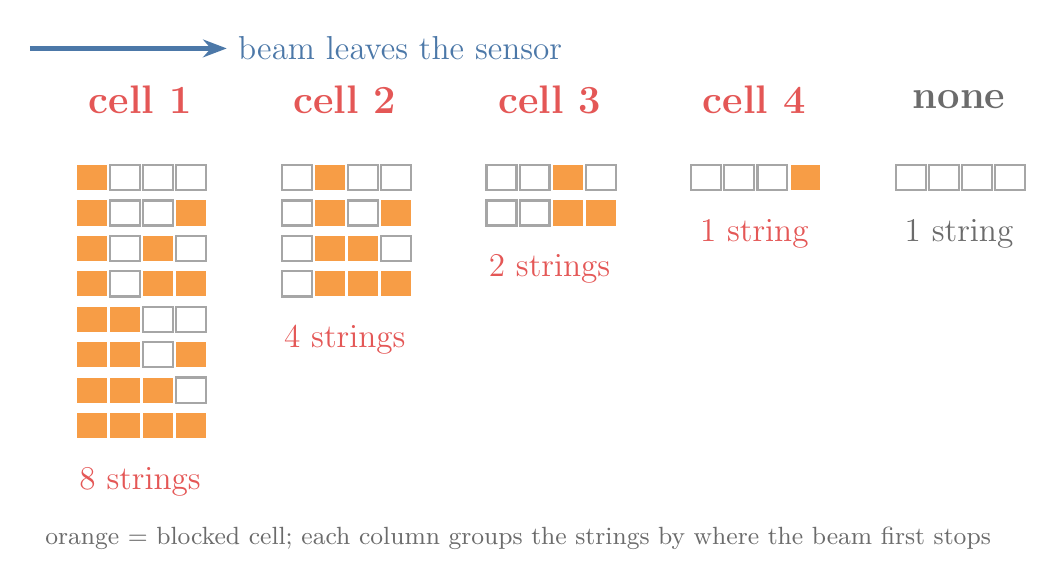
\begin{tikzpicture}[every node/.append style={font=\large}]
  \def\cols{{0,2.6,5.2,7.8,10.4}}
  % group 1
  \node[title, cred] at (0.8,0.7) {cell 1};
  \foreach \s [count=\j] in {{1,0,0,0},{1,0,0,1},{1,0,1,0},{1,0,1,1},{1,1,0,0},{1,1,0,1},{1,1,1,0},{1,1,1,1}} {
    \edef\bits{\s} \cellrow{0}{-\j*0.45} }
  \node[cred] at (0.8,-4.15) {8 strings};
  \node[title, cred] at (3.4,0.7) {cell 2};
  \foreach \s [count=\j] in {{0,1,0,0},{0,1,0,1},{0,1,1,0},{0,1,1,1}} { \edef\bits{\s} \cellrow{2.6}{-\j*0.45} }
  \node[cred] at (3.4,-2.35) {4 strings};
  \node[title, cred] at (6.0,0.7) {cell 3};
  \foreach \s [count=\j] in {{0,0,1,0},{0,0,1,1}} { \edef\bits{\s} \cellrow{5.2}{-\j*0.45} }
  \node[cred] at (6.0,-1.45) {2 strings};
  \node[title, cred] at (8.6,0.7) {cell 4};
  \foreach \s [count=\j] in {{0,0,0,1}} { \edef\bits{\s} \cellrow{7.8}{-\j*0.45} }
  \node[cred] at (8.6,-1.0) {1 string};
  \node[title, cgrey] at (11.2,0.7) {none};
  \foreach \s [count=\j] in {{0,0,0,0}} { \edef\bits{\s} \cellrow{10.4}{-\j*0.45} }
  \node[cgrey] at (11.2,-1.0) {1 string};
  \draw[-{Stealth[length=3mm]}, cblue, line width=1.6pt] (-0.6,1.35) -- (1.9,1.35) node[right, cblue] {beam leaves the sensor};
  \node[note, anchor=north] at (5.6,-4.6) {orange = blocked cell; each column groups the strings by where the beam first stops};
\end{tikzpicture}
\end{document}
